\documentclass[10pt,conference,compsocconf]{IEEEtran}

\usepackage{hyperref}
\usepackage{graphicx}	% For figure environment
\usepackage{amsmath}

\newcommand{\cN}{\mathcal{N}}
\newcommand{\argmax}{\mathrm{argmax}}
\begin{document}

\title{Project 2 Machine Learning: Road Segmentation}

\author{
   Kirtan Padh, Damian Straszak, Jakub Tarnawski\\
    
  \textit{Department of Computer Science, EPFL, Switzerland}\\
  {\it Kaggle team: haggle on kaggle} \\
}

\maketitle

\begin{abstract}
We propose a machine learning model which uses Convolutional Neural Networks(CNN) to extract roads from satellite images. We give a roadmap of how we arrived at our final model and describe it it detail, followed by the description of some advanced post processing steps using integer programming that we used to improve the accuracy. Our predictions based on this model achieve an F1 score of $91.704\%$ on the kaggle leaderboard.
\end{abstract}

\section{Introduction}
The problem statement we chose for the project is that given a satellite image taken from google maps, we need to classify each pixel as either road or background. We are given a training set of $100$ images of size $400 \times 400$ pixels, with each pixel classified appropriately. The testing set consists of $50$ images of size $608 \times 608$ pixels. This is a well studied problem in literature. Wang et al.\cite{wang16} give a comparison of the several different types of methods that have been used to tackle this problem.

Our methodology towards solving the problem is as follows.

\section{Methodology}
We are given two baseline methods for the project. One is a simple linear regression model and the other is a CNN with two convolutional layers and 2 pooling layers. We begin by trying simple classification techniques such as logistic regression and move on to more advanced techniques such as ADA boost and gradient boost and finally the baseline CNN given to us. Since we have access to a cluster on which we can train our model, we decide to first find a model which gives a reasonable good F1 score on the PC and then train it on the cluster.

Table~\ref{baseline} summarizes the validation accuracies we obtain when trying increasingly complex classification models, but without doing a great amount of optimization on any of them. The F1 scores obtained are by doing a small grid search for each of the models around the default parameters and cross-validating. 
\begin{figure}[h!]
\center
\begin{tabular}{ l | c  }
  Model & F1 score $\pm$ standard deviation  \\
  \hline
  Logistic Regression (LR) & $65.9 \pm 2.311e^{-3}$  \\
  LR (polynomial basis) & $67.0 \pm 0.65$  \\
  ADA Boost & $26.37 \pm 1.26$ \\
  Gradient boost & $23.3 \pm 2.1$
\end{tabular}
\caption{Baseline comparison of classification models implemented and crossvalidated using scikit-learn}
\label{baseline}
\end{figure}
It seems that these simple classification techniques are not able to achieve a high F1 score. Some of these models achieve high accuracy of around $75\%$, but the resulting F1 score is still low.

We now move to discussing the provided baseline CNN. Refer to Section~\ref{basic} for details on how it is constructed.  In Figure~\ref{lr} we have plotted validation scores obtained for this method when running it with standard parameters. We used a patch size of $16$ (for details on this and other parameters see Section~\ref{basic}). We have also tested patch sizes of $8$ and $4$, but the results were significantly worse.
\begin{figure}
 \center
 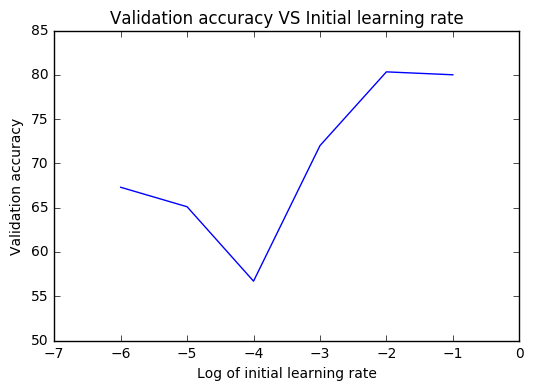
\includegraphics[scale=0.5]{lr.png}
 \caption{Validation accuracy VS Initial learning rate}
 \label{lr}
\end{figure}

When the learning rate is $0.01$ we obtain an F1 score of $83.3\%$, which is much better than the models we saw previously. The loss curves are plotted in Figure~\ref{loss} for different values of initial learning rates to get a better comparison along with the F1 score.  
\begin{figure}
 \center
 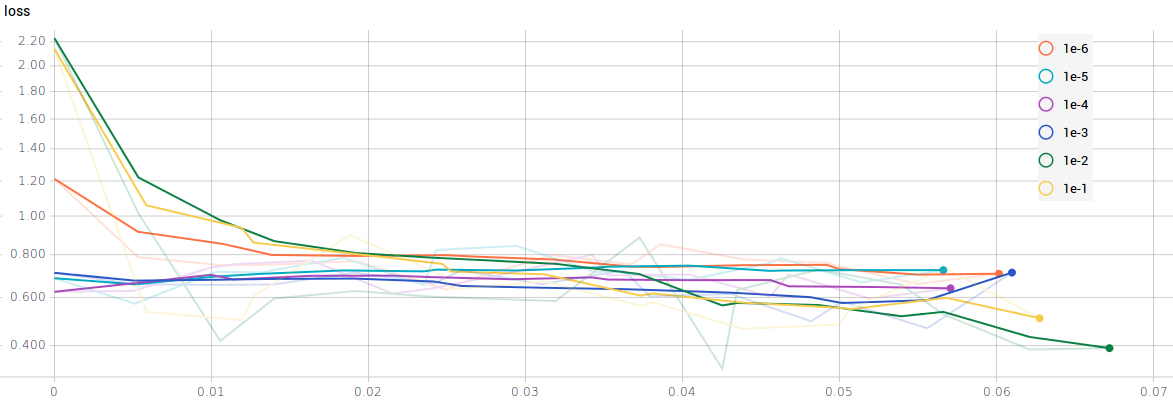
\includegraphics[scale=0.2]{loss_curves.png}
 \caption{The plot of the loss curves for each value of initial learning rate we tried. x-axis shows (number of iterations)/1000}
 \label{loss}
\end{figure}
We observe that while both $0.1$ and $0.01$ achieve a good F1 score, the loss curve for the value $0.01$ seems to be better as it is still decreasing with the increasing iteration, while the one for $0.1$ is starting to get stable. Hence we choose the initial learning rate to be $0.01$.


In the above we used some simple rounding methods to get the final predictions from the output of the CNN. It turns out that one can be more careful and creative when rounding these (as we call them) heat maps to actual solutions. Thus, we divide the process of obtaining prediction into two disjoing parts:
\begin{enumerate}
\item obtaining a heat map (discussed in Section~\ref{model}),
\item the post-processing phase (discussed in Section~\ref{post}).
\end{enumerate}
The latter can be implemented as some simple treshold rounding, however several other, more involved methods can be proposed for this part. Indeed in Section~\ref{post} we propose a way to obtain final predictions from the heat maps by solving a non-trivial optimization problem formulated as an integer program. 





  
\section{Obtaining heat maps}\label{model}
In this section we are going to describe the first component of our framework which is a method to transform a given input image into (how we call it) a {\it Road Heat Map}. More precisely suppose an image $I$ is given of dimensions $n\times n$, then the output of our method is an array $x\in [0,1]^{n\times n}$ with the intent that $x(i,j)$ corresponds to the probability that the pixel $(i,j)$ is part of a road. Clearly this is the essential part of the task and the accuracy here crucially affects the final accuracy of our method, no matter how we proceed after that. 

\subsection{Basic CNN}\label{basic}
The provided sample code {\it tf\_aerial\_images.py} of a Convolutional Neural Network for solving this task serves as good starting point for our final approach. Let us describe it briefly here. To compute a prediction for a given input picture of dimension $n\times n$, the picture is first divided into $\frac{n}{16} \times \frac{n}{16}$ chunks of size $16 \times 16$ each. Subsequently, every such chunk $C$ is being input into a neural network $\cN$, which outputs a number $p(C) \in [0,1]$ which is then used as the heat map value for the corresponding $16\times 16$ chunk. What is left to explain is how is $\cN$ constructed and how is it trained. The network $\cN$ has the following layers: (\textit{Convolutional, Max Pooling}) repeated twice in this order. To calculate  losses, the cross entropy function is used. The network  is trained using training pairs $(x,y)$ (input and output) of the form: $x$ is a $16\times 16$ chunk, part of a training picture and $y \in \{0,1\}$ is a suitably rounded mean of the corresponding ground truth chunk.  

To deal with the network $\cN$ efficiently, the {\it TensorFlow} library is used. In particular, this provides us with a ready-to-apply optimization primitive {\it MomentumOptimizer}. The learning rate is chosen as discribed in the previous section.

\subsection{Big CNN}
Our way of obtaining heat maps builds upon the approach described above, but includes several new insights and modifications which we are going to describe below and briefly discuss how do they affect the results and accuracy.

The first modification we employ concerns the general philosophy how the heat map is obtained. Note that in the basic approach above, the heat map is ``discrete'' in the sense that it is constant on $16 \times 16$ chunks. Another disadvantage is that the result for a single chunk depends \emph{only} on the pixels within it, not at all on the neighboring ones, whereas in reality such a prediction cannot be performed locally.

To fix these issues we propose and implement a different method for computing the heat map. For every pixel $(i,j)$ in the image we take its square neighborhood of size $48\times 48$ and feed it into a new neural network $\cN'$ to get a single value $p'\in [0,1]$ which determines the value of the corresponding entry $(i,j)$ in the heat map. By this design we get a much ``smoother'' heat map, which also does not suffer so much from the ``locality'' issue, as the value of a pixel is determined by looking at a quite large neighborhood of it. To see a sample on how much improvement does it yield, refer to Figure~\ref{fig:smallbig}.
\begin{figure}
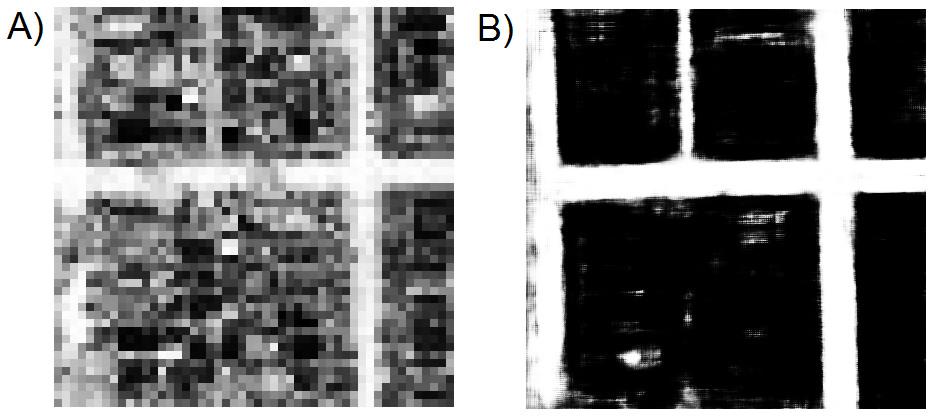
\includegraphics[scale=0.42]{smallbig.png}
\caption{The difference in quality between heat maps computed using the Basic Neural Network A) and the Big Neural Network B).}
\label{fig:smallbig}
\end{figure}
Note that such a change in the model introduces some issues with efficiency. Indeed the network $\cN'$ is significantly larger than $\cN$ and also the number of predictions which need to be performed increases roughly $16^2=256$ times, when compared to the previous model. Further, also training such a network becomes computationally quite demanding. We obtain reasonable running times by taking advantage of a workstation with 20 cores and using the parallelization power {\it TensorFlow} provides. In particular, for the latter, we coded the predictions to run in batches of $32$, which allows them to be executed in parallel at multiple cores. It turns out that $32$ is essentially the optimal number here, since increasing it to $64$ requires enormous amounts of memory and reducing it to $16$ makes the process a little slower.

\subsection{Diagonal Roads}
One of the issues which appears after training our model on the training data  only  is that the roads, which are diagonal in the testing data are hardly recognized. This might be because a typical road in the training data is either vertical or horizontal, which is then ``learned'' by the network as correct. For an example see Figure~\ref{fig:diagonal}.
\begin{figure}
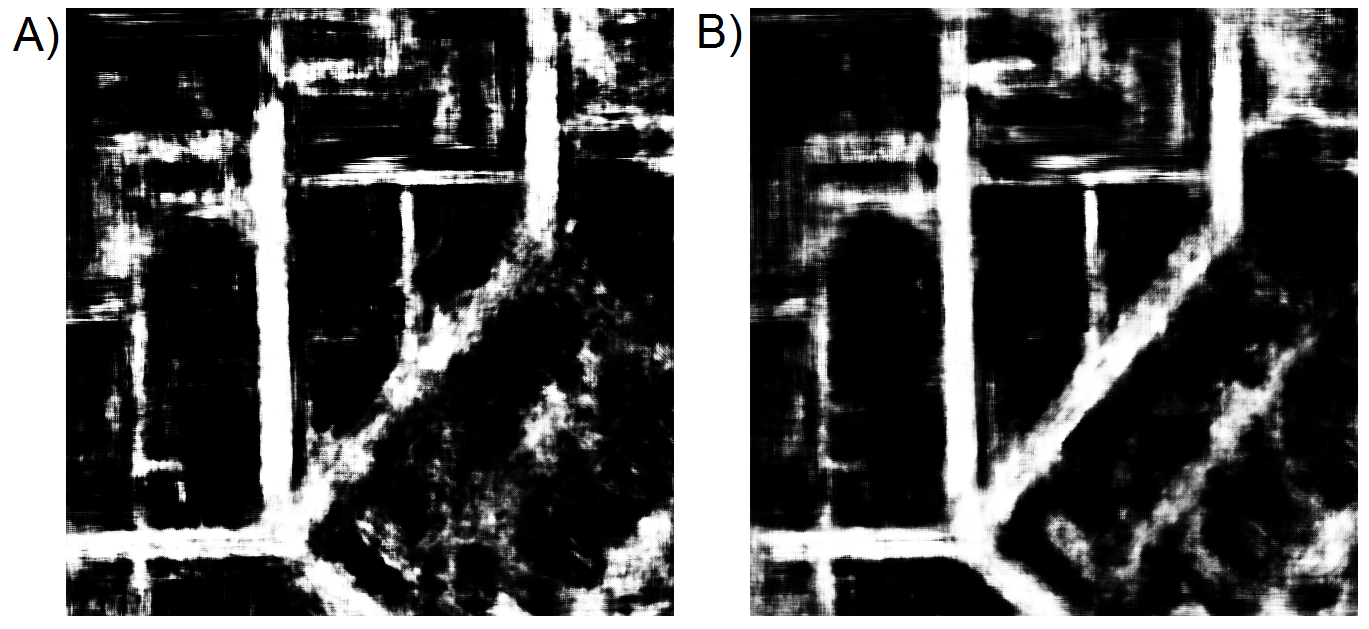
\includegraphics[scale=0.3]{diagonal.png}
\caption{The results of predictions when trained on just the training data A) and after adding rotated images B).}
\vspace{2mm}
\label{fig:diagonal}
\end{figure}
To get around this problem we add several random rotations of the training images to the training data. This has the desired effect of making the ``confidence'' of diagonal and non-diagonal predictions equal. Indeed without rotated pictures in the training data, the vertical and horizontal roads were typically detected with a (too) large confidence while the diagonal ones were either very blurry or nonexistent. After this manipulation there is symmetry among different directions of roads in terms of intensity in the heat map.

\subsection{Overfitting}
To control overfitting we were performing validation over $30\%$ of the training data. Indeed we encountered significant overfitting when using different parameters for the model of our Neural Network. When using chunks of size $64$ (instead of $48$ as we use in the final version) the difference between the average prediction scores for instances used for training and for instances outside of the training set reached roughly $0.1$. In the current version it is no more than $0.02$. 

The weak form of validation we use is mainly because of efficiency reasons. While for the Basic Neural Network we were able to run full $K-$fold cross validation for $K=4$, it is no more feasible for the Big Network (because training is very time consuming). Since the results we were obtaining were much better for the Big Network, we decided to stick to it and relax the validation method to a weaker one.



\section{The Post-Processing Phase}\label{post}



In the previous step, we have obtained, for each pixel $(i,j)$, an estimate $p = p_{ij} \in [0,1]$ of whether this pixel of the (high-resolution) ground truth is white (i.e., a road). We interpret this number as a probability. In this section, we discuss how to convert this to a black or white value for each $16 \times 16$ patch; we call this process \emph{rounding} or \emph{post-processing}. We will treat each patch separately and focus on a single patch.

\subsection{The simple algorithm}

A simple method is just to choose a threshold $t$ (typically $t = 0.25$ since this is how the ground truth is generated)\footnote{In our code, $t$ is called \textit{foreground\_threshold}.} and, for each patch, take the mean of the estimated values $m = \frac{\sum p_{ij}}{16 \cdot 16}$. Then, output white iff $m > t$. The parameter $t$ can be optimized to get good validation scores.



% A downside to this approach is that, intuitively, we are discarding the structure given by the patch by just taking its mean. 
\subsection{Integer Programming}

We opt for a more involved approach. First, we estimate the likelihood $\ell \in [0,1]$ of the patch. We would like to take those patches with $\ell > 0.5$. Intuitively, we want it to satisfy that if all pixels have $p \approx 0.25$, then $\ell \approx 0.5$ (since this is the point at which we are not sure whether to take the patch). The same should hold if we have a $0.25$ fraction of pixels with $p = 1$ and the rest have $p = 0$.

One method to get $\ell$ is to compute the mean $m$ and then set $\ell(m)$ to be a piecewise linear function with $\ell(0) = 0, \ell(t) = 0.5, \ell(1) = 1$.

Another one is to assume that each pixel is an \emph{independent} $p$-biased coin flip. Then, we can use dynamic programming to compute, for each $k \in \{0, ... 16 \cdot 16\}$ the exact probability that $k$ pixels are white. We take the probability that the number of white pixels is above the threshold.\footnote{See the code in \texttt{estimate\_probability.py} for details, including the recurrence relation for the dynamic programming.}

In practice, we choose the first method because of its simplicity and speed.\footnote{Unfortunately, in Python, this dynamic programming uses about 2-3 seconds per image (even if implemented using NumPy), which makes it difficult to try many hyperparameters.}

Now that we have the likelihood $\ell_v$ for each patch $v$, we develop our Integer Programming approach. Assume that patches are independent. That is, the likelihood of a set of patches is the product of the likelihoods of picking each patch in the set (as well as not picking each patch not in the set). We would like to pick the maximum-likelihood set of patches.


Let $V$ be the set of patches indexed by $v$; thus we want:
\begin{align*}
\argmax_{X \subseteq V} \ell(X) &= \argmax_{X \subseteq V} \prod_{v \in X} \ell_v \prod_{v \in V \setminus X} (1 - \ell_v)
\end{align*}
taking logarithms, we obtain that $\argmax_{X \subseteq V} \log \ell(X) $ equals
\begin{align*}
& \argmax_{X \subseteq V} \sum_{v \in X} \log \ell_v + \sum_{v \in V \setminus X} \log (1 - \ell_v) \\
=& \argmax_{X \subseteq V} \sum_{v \in V} \log (1 - \ell_v) + \sum_{v \in X} \log (\ell / (1 - \ell_v)) \\
=& \argmax_{X \subseteq V} \sum_{v \in X} \log (\ell_v / (1 - \ell_v)) \\
=& \argmax_{X \subseteq V} \log (\ell_v / (1 - \ell_v)) x_v
\end{align*}
where $x_v \in \{0,1\}$ denotes whether we choose $v$ or not. Unsurprisingly, this is maximized by taking $x_e = 1$ iff $\log(\ell_v / (1 - \ell_v)) > 0$, which is equivalent to $\ell_v > 0.5$.

However, the fun is only starting: now we can add extra constraints or modify the objective function of this Integer Programming formulation.

For one, we notice that the white region in the ground truth is always connected (at least if we add the border of the image). Indeed, we would like to get rid of disconnected small white segments in our answers, as they are usually wrong.

Second, we want our output to look ``smooth'', without jagged edges (since the ground truth looks like this). We quantify this as follows: we put a penalty on each pair of neighbouring cells which have different colours, thus seeking to minimize the length of the border. Namely, we define a variable $z_{ab} = |x_a - x_b|$ for each two neighbouring cells $a$ and $b$, and add $- \alpha \sum_{ab} z_{ab}$ to the objective function, where $\alpha > 0$ is a parameter to be chosen.\footnote{Called \texttt{border\_penalty} in the code.}

For the connectivity, we define a graph: the vertices are the cells, adjacent ones have edges between them, and we add a root vertex which is connected to the border cells. In this graph, we require that there should exist a flow from the root to the set of vertices $v$ with $x_v = 1$, which sinks flow into each such vertex. The flow may only be positive between cells with $x_v = 1$. This can be accomplished by adding linearly many variables and constraints to the program, and enforces that there is no component of white cells disconnected from the root.\footnote{A brief argument for this is as follows: if there was, then the flow must reach these vertices in order to have negative flow conservation, but this is impossible because there is no way to reach this component from the root.}

We can solve this integer program using the Gurobi optimizer.\footnote{It seems to be of just the right size to be feasible, because it is solved in (usually) a few seconds.} This leaves us with optimizing two hyperparameters, which are $t$ and $\alpha$. The best score we are able to get using this method is $0.798$ using the local validation set and $0.917$ on the public Kaggle scoreboard, using a setting of $t = 0.28$ and $\alpha = 0.28$. While this is not a large improvement over the simple method, where we score $0.797$ locally and $0.915$ on Kaggle using $t = 0.28$, we think that this method is interesting and has the potential to yield higher scores if pushed further (perhaps by optimizing hyperparameters when using the dynamic programming method of obtaining the likelihoods $\ell$). A similar method was also used by \cite{turetken2013reconstructing,turetken2016reconstructing} for delineation of curvilinear structures in images (including road networks).\footnote{These papers are however somewhat hindered by the size of their Integer Programming formulations, which is quadratic; on the other hand, we managed to obtain a linear-sized formulation, which makes it possible to solve the $38 \times 38$ grid instance in seconds.}





\bibliographystyle{IEEEtran}
\bibliography{literature}

% TODO: cite this http://www.cs.toronto.edu/~fritz/absps/road_detection.pdf (just that there is a history of doing road semgnetation with NNs)

\end{document}
